%%%%%%%%%%%%%%%%%%%%%%%%%%%%%%%%%
\newpage
%%%%%%%%%%%%%%%%%%%%%%%%%%%%%%%%%
\section{Convolution introduction}

\subsection*{Resources}
\begin{itemize}
    \item Video lecture 8 starting at 32:15: \url{https://youtu.be/wUT1huREHJM?t=32m15s}
\end{itemize}

\subsection*{Comment}
Here we expand our study to convolution; a powerful function for processing signals. Convolution is not immediately intuetive, but Prof. Osgood provides an excellent introduction.

\subsection*{Challenge}
Make notes following the above video deriving the formula relating convolution in the frequency and time domains.

\timebox




%%%%%%%%%%%%%%%%%%%%%%%%%%%%%%%%%
\newpage
%%%%%%%%%%%%%%%%%%%%%%%%%%%%%%%%%
\section{Filtering}

\subsection*{Resources}
\begin{itemize}
    \item Video lecture 9 until 24:15: \url{https://www.youtube.com/watch?v=NrOR2qMVWOs}
\end{itemize}

\subsection*{Comment}
The above video includes an excellent example of using fourier analysis in a scientific context, including its application in filters.

The challenge below asks you to watch to 24:15, however after this point he goes on to describe the futility of trying to visualise convolution in the time-domain. Nevertheless, the graphics on convolution on Wikipedia [1] (especially these: [2a,b]) I think go some way to visualising what's happening in the time-domain.

1: \url{https://en.wikipedia.org/wiki/Convolution}\\
2a: \url{https://en.wikipedia.org/wiki/Convolution\#/media/File:Convolution_of_box_signal_with_itself2.gif}\\
2b: \url{https://en.wikipedia.org/wiki/Convolution\#/media/File:Convolution_of_spiky_function_with_box2.gif}

For your reference, turbidity standards of 5, 50, and 500 Nephelometric Turbidity Units (left to right respectively) are shown here:\\
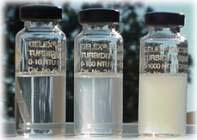
\includegraphics{turbidity.png}\\
\emph{Source: \url{https://en.wikipedia.org/wiki/Turbidity}}

\subsection*{Challenge}
1. Take notes following the above video until 24:15. There is a lot of useful information here. The questions below highlight the key points that I want you to understand, however they do not cover everything, so please be sure to follow the video.

2. Using a few sentences and diagrams, describe an ideal low-pass, high-pass and band-pass filter. How can they be applied in the frequency domain to influence the signal in the time-domain?

3. Write a few sentences and equations describing how convolution in the time-domain is related to signal multiplication in the frequency-domain.

\timebox


\iffalse
%%%%%%%%%%%%%%%%%%%%%%%%%%%%%%%%%
\newpage
%%%%%%%%%%%%%%%%%%%%%%%%%%%%%%%%%
\section{Convolution with a window function}

\subsection*{Comment}
To the ``signal'' here is $g(t-\tau)$ and the ``window function'' is $f(\tau)$.

\subsection*{Challenge}
1. Consider that you have a (somewhat unrealistic but mathematically manageable) input signal that varies as $g(t-\tau)=(t-\tau)^2$ with time. 

Obtain the convolution of the signal $(f \star g)(t)$ with a window function (essentially a low-pass filter)
\begin{equation}
    f(\tau)=
    \begin{cases}
        1 & \text{for } -1/2 < \tau < 1/2\\
        0 & \text{otherwise}
    \end{cases}
\end{equation}

2. Compare the answer above when $t=0$ with direct integration of $\tau^2$ between $-1/2$ and $1/2$. Why are they the same?

\subsection*{Solution}
\hash{ppp}{290253}

\timebox




%%%%%%%%%%%%%%%%%%%%%%%%%%%%%%%%%%
%\newpage
%%%%%%%%%%%%%%%%%%%%%%%%%%%%%%%%%%
%\section{Convolution with a continuous function}
%
%\subsection*{Challenge}
%Consider that you have a (somewhat unrealistic but mathematically manageable) input signal that varies with time $\tau$ as $f(\tau)=\tau$.  Apply a filter to the signal that is defined at time $t$ as $e^{-|t|}$.
%
%\emph{Hint: $\int_{-\infty}^{\infty} \text{(even function)} = 2 \int_{0}^{\infty} \text{(even function)}$.}
%
%To check your answer, substitute $t=1$ into your final answer.
%
%\subsection*{Solution}
%\hash{qqq}{e48f28}
%
%\timebox




%%%%%%%%%%%%%%%%%%%%%%%%%%%%%%%%%%
%\newpage
%%%%%%%%%%%%%%%%%%%%%%%%%%%%%%%%%%
%\section{Inequalities}
%
%\subsection*{Challenge}
%1. Re-write $-1/2 < t - \tau$ in the form $f(\tau) < t$ replacing $f(\tau)$ with appropriate expressions.
%
%2. Re-write $t - \tau < 1/2$ in the form $t < f(\tau)$ replacing $f(\tau)$ with appropriate expressions.
%
%3. Re-write $-1/2 < t - \tau < 1/2$ in the form $f(\tau) < t < g(\tau)$ replacing $f(\tau)$ and $g(\tau)$ with appropriate expressions.
%
%\subsection*{Solution}
%To check your solutions, substitute $\tau=1/2$ into the final expressions:
%
%1. $f(1/2)$: \hash{kkk}{115edb}\\
%2. $f(1/2)$: \hash{mmm}{6d64cd}\\
%3. $f(1/2)$: \hash{nnn}{414d80} and $g(1/2)$: \hash{ooo}{3ec4d7}
%
%\timebox




%%%%%%%%%%%%%%%%%%%%%%%%%%%%%%%%%%
%\newpage
%%%%%%%%%%%%%%%%%%%%%%%%%%%%%%%%%%
%\section{Touching window functions}
%\label{sec:touchingwindows}
%
%\subsection*{Challenge}
%1. Consider two window functions $f$ and $g$.
%\begin{equation}
%    f(\tau)=
%    \begin{cases}
%        1 & \text{for } -1/2 < \tau < 1/2\\
%        0 & \text{otherwise}
%    \end{cases}
%\end{equation}
%\begin{equation}
%    g(t-\tau)=
%    \begin{cases}
%        1 & \text{for } -1/2 < t-\tau < 1/2\\
%        0 & \text{otherwise}
%    \end{cases}
%\end{equation}
%You can imagine a fixed window function $f$ and a shiftable window-function $g$ (depending on the value of $t$). What is the value of $t$ in the following situations?
%
%a) The left side of window $f$ and the right side of window $g$ are touching.\\
%b) Complete overlap of windows $f$ and $g$.\\
%c) The right side of window $f$ and the left side of window $g$ are touching.
%
%2.\\
%a) Write a function that describes the position of the left-hand-side of window function $g$ at time $t$.\\
%b) Write a function that describes the position of the right-hand-side of window function $g$ at time $t$.\\
%To check your answers, substitute $t=1$ into your expressions.
%
%\subsection*{Solution}
%1.a) \hash{rrr}{1e3803}\\
%1.b) \hash{sss}{171271}\\
%1.c) \hash{ttt}{95acc3}\\
%
%2.a) \hash{uuu}{e27eca}\\
%2.b) \hash{vvv}{23da5b}
%
%\timebox




%%%%%%%%%%%%%%%%%%%%%%%%%%%%%%%%%
\newpage
%%%%%%%%%%%%%%%%%%%%%%%%%%%%%%%%%
\section{Convolution of two window functions}

\subsection*{Challenge}
%1. Show that the convolution of the two window functions in challenge \ref{sec:touchingwindows} in the time-domain results in the triangle function
%\begin{equation}
%    h(t)=
%    \begin{cases}
%        1+t & \text{for } 1 < t < 0\\
%        1-t & \text{for } 0 < t < 1\\
%        0 & \text{otherwise}
%    \end{cases}
%\end{equation}

In challenge \ref{sec:tophat} you calculated the spectrum of a window function. Imagine here you have two window functions $f(t)$ and $g(\tau)$.

\begin{equation}
    f(t)=
    \begin{cases}
        1 & \text{for } |t| < 1/2 \\
        0 & \text{for } |t| > 1/2
    \end{cases}
\end{equation}

\begin{equation}
    g(\tau)=
    \begin{cases}
        1 & \text{for } |\tau| < 1/2 \\
        0 & \text{for } |\tau| > 1/2
    \end{cases}
\end{equation}

1. Calculate the frequency-domain spectrum of the convolution of the two window functions.

2. Deduce (without calculation) what the resulting function is in the time-domain.

\subsection*{Solution}
To check your answer, substitute $s=1$ into your answers

1. 0.71

2. \hash{www}{9a90c0}

\timebox
\fi
